\documentclass[pdftex,12pt,a4paper]{report}

\usepackage[portuguese,english]{babel}
\usepackage[T1]{fontenc} 
\usepackage[utf8]{inputenc}
\usepackage[pdftex]{graphicx}
\usepackage{minitoc}
\usepackage{hyperref}
\usepackage{indentfirst}
\usepackage[compact]{titlesec}
\usepackage{fancyhdr}
\usepackage{caption}
\usepackage{pgfplots}
\usepackage{pgfplotstable}
\usepackage{fixltx2e}
\usepackage{mathtools}
\usepackage{fancyhdr}
\usepackage{listings}
\usepackage{color}
\usepackage{sverb}

\definecolor{Black}{rgb}{0.0, 0.0, 0.0}
\definecolor{Blue}{rgb}{0.0, 0.0, 1.0}
\definecolor{DarkGreen}{rgb}{0.0, 0.42, 0.24}
\definecolor{Red}{rgb}{0.89, 0.0, 0.13}

\lstset{
  breaklines=true,                                     % line wrapping on
  language=SQL,
  frame=ltrb,
  framesep=5pt,
  basicstyle=\normalsize,
  keywordstyle=\ttfamily\color{Blue},
  identifierstyle=\ttfamily\color{Black}\bfseries,
  commentstyle=\color{DarkGreen},
  stringstyle=\ttfamily\color{Red},
  showstringspaces=ture
}

\pagestyle{fancy}
\renewcommand*\thesection{\thechapter\arabic{section}}
\newcommand{\HRule}{\rule{\linewidth}{0.5mm}}
\begin{document}

\begin{titlepage}

\begin{center}


\includegraphics[width=0.15\textwidth]{./logo}\\[0.5cm]    

\textsc{\large Universidade de Aveiro \\[1cm]\large departamento de electrónica, telecomunicações e informática}\\[1cm]

\textsc{\large{42532}\large - Base de Dados \\[1cm]}

\HRule \\[0.5cm]
{ \huge \bfseries Football Club}\\[0.4cm]
{ \large \bfseries Trabalho Prático Final}\\[0.4cm]
\HRule \\[1cm]

\textsc{\small{8240 - MESTRADO INTEGRADO EM ENGENHARIA DE COMPUTADORES E TELEMÁTICA}}\\[1cm]

\begin{minipage}{0.4\textwidth}

\begin{flushleft} \large
\href{mailto:rafael.ferreira@ua.pt}{António Rafael da \\ Costa Ferreira }
 \small{\\NMec: 67405 | P4G5}
\end{flushleft}
\end{minipage}
\begin{minipage}{0.4\textwidth}

\begin{flushright} \large
\href{mailto:rodrigocunha@ua.pt}{Rodrigo Lopes \\ da Cunha}
\small{\\NMec: 67800 | P4G5}
\end{flushright}
\end{minipage}\\[1cm]

{\large Docente: Carlos Manuel Azevedo Costa   }\\[0.5cm]

\vfill

{\large Junho de 2015 \\ 2014-2015}

\end{center}

\end{titlepage} %Titulo do Relatorio
\renewcommand{\headrulewidth}{0pt}

%Cabeçalhos de rodapé
\fancyhead{}
\fancyfoot{}
\lhead{Football Club - Trabalho Prático Final}
\rhead{BD - 2014/2015}
\lfoot{\textit{P4G5} \\ Rafael Ferreira nmec: 67405 \\ Rodrigo Cunha nmec: 67800}
\rfoot{\thepage}

%Renomear Comandos
\renewcommand*\contentsname{Conteúdos}
\renewcommand*\figurename{Figura}
\renewcommand*\tablename{Tabela}

%Conteúdos, dar paragrafo
\tableofcontents
%Headers
\renewcommand{\headrulewidth}{0.15pt}
\renewcommand{\thechapter}{}

\clearpage

\section{Introdução}
% o que, porquê e o objetivo
O trabalho proposto para o projeto da unidade curricular de Base de Dados é uma plataforma de gestão de um clube de futebol. Usando os conhecimentos adquiridos, propôs-se o desenvolvimento deste projeto visto que o futebol é uma modalidade mundial, envolvendo vários tipos de interesse. 

O objetivo desta base de dados desenvolvida é permitir a gestão de todos os processos de um clube de futebol, como será visto mais à frente.

Além de se ter desenvolvido esta base de dados, desenvolveu-se uma aplicação WPF C\# para permitir a manipulação dos dados da base de dados de forma mais simplificada para um utilizador final.

Esta base de dados deve fornecer ferramentas que permitam a criação, remoção, alteração e consulta da base de dados de forma segura, eficiente e robusta.

O relatório reflete todos os passos e decisões tomadas na criação da base de dados que sustenta o projeto bem como uma descrição das capacidades da aplicação desenvolvida para o cliente.

Para a criação deste projeto foi seguido o processo leccionado nas aulas, sendo estas as seguintes fases do processo: análise de requisitos, desenho conceptual, desenho do esquema lógico, desenho do esquema físico e administração.

\newpage
\section{Análise de Requisitos}

A análise de requisitos foi uma das partes mais importantes do processo de concepção do projeto uma vez que ajudou a ter uma visão clara do que o sistema teria de suportar. Após realizado um "brainstorming", estas são as características que o sistema deve suportar:

Uma \textbf{pessoa} é identificada por um nome, B.I. (sendo que este B.I. é único), endereço, NIF, Sexo, Data de Nascimento e Nacionalidade. Esta pessoa pode ser uma Pessoa que pertença ao pessoal interno do clube (Staff) ou ser um sócio do clube. 

Uma \textbf{pessoa interna} ao clube tem salário e um ID que é automaticamente atribuído e o identifica dentro do clube.

Um \textbf{sócio do clube} tem um nº de sócio, o ano até que as suas cotas estão pagas (são cotas anuais) e um valor de cotas que tem de pagar todos os anos. Um sócio pode ter ou não um \textbf{lugar anual}, tendo este, um valor, data de início, duração, Nº Lugar e Nº Fila e ID da secção.

Um \textbf{lugar} tem um nº de lugar e fila. Uma \textbf{secção} tem um ID de secção e tipo. 

Um \textbf{jogador} é uma pessoa interna ao clube e é identificado com um ID da federação, peso e altura. Este joga em equipas do clube.

Um \textbf{treinador} é uma pessoa interna do clube e é identificado com um ID da federação e cargo. Este tem equipas do clube.

Uma \textbf{equipa} tem uma idade máxima de jogadores que podem pertencer à mesma e um nome único.

Uma equipa pode ter \textbf{treinos} que são caracterizados por uma data e uma hora e são realizados num determinado campo.

Um \textbf{campo} tem um endereço e um ID.

Uma pessoa interna ao clube (\textbf{Staff}) tem um cargo e pode trabalhar um Departamento.

Um \textbf{departamento} tem um endereço, ID de departamento e um nome.

\newpage

Foram também registadas algumas especificações para o desenho conceptual:

- Uma pessoa pode ser um sócio ou uma pessoa interna.

- Uma pessoa interna ao clube pode ser um jogador, um coach ou um membro do staff.

- Um sócio pode ter vários lugares anuais mas um lugar anual apenas pertence a um membro.

- Um lugar pode ter vários lugares anuais mas um lugar anual apenas tem um lugar.

- Uma secção pode ter vários lugares mas um lugar pode ter apenas uma secção.

- Um membro do staff apenas pode trabalhar num departamento e um departamento pode ter vários membros do staff.

- Um jogador pode jogar em várias equipas e uma equipa pode ter vários jogadores.

- Um treinador pode jogar em várias equipas e uma equipa pode ter vários treinadores.

- Uma equipa pode ter vários treinos mas um treino apenas pode ter uma equipa.

- Um treino apenas pode ter um campo e um campo pode ter vários treinos.

\newpage
\section{Diagrama entidade relação}
Depois da análise de requisitos desenhou-se o diagrama entidade relação do nosso sistema. Este desenho foi descrito através de um diagrama ER\ref{fig:eer}. No diagrama, foram definidas entidades, atributos, relações, cardinalidades e dependências.

\begin{figure}[!htb]
 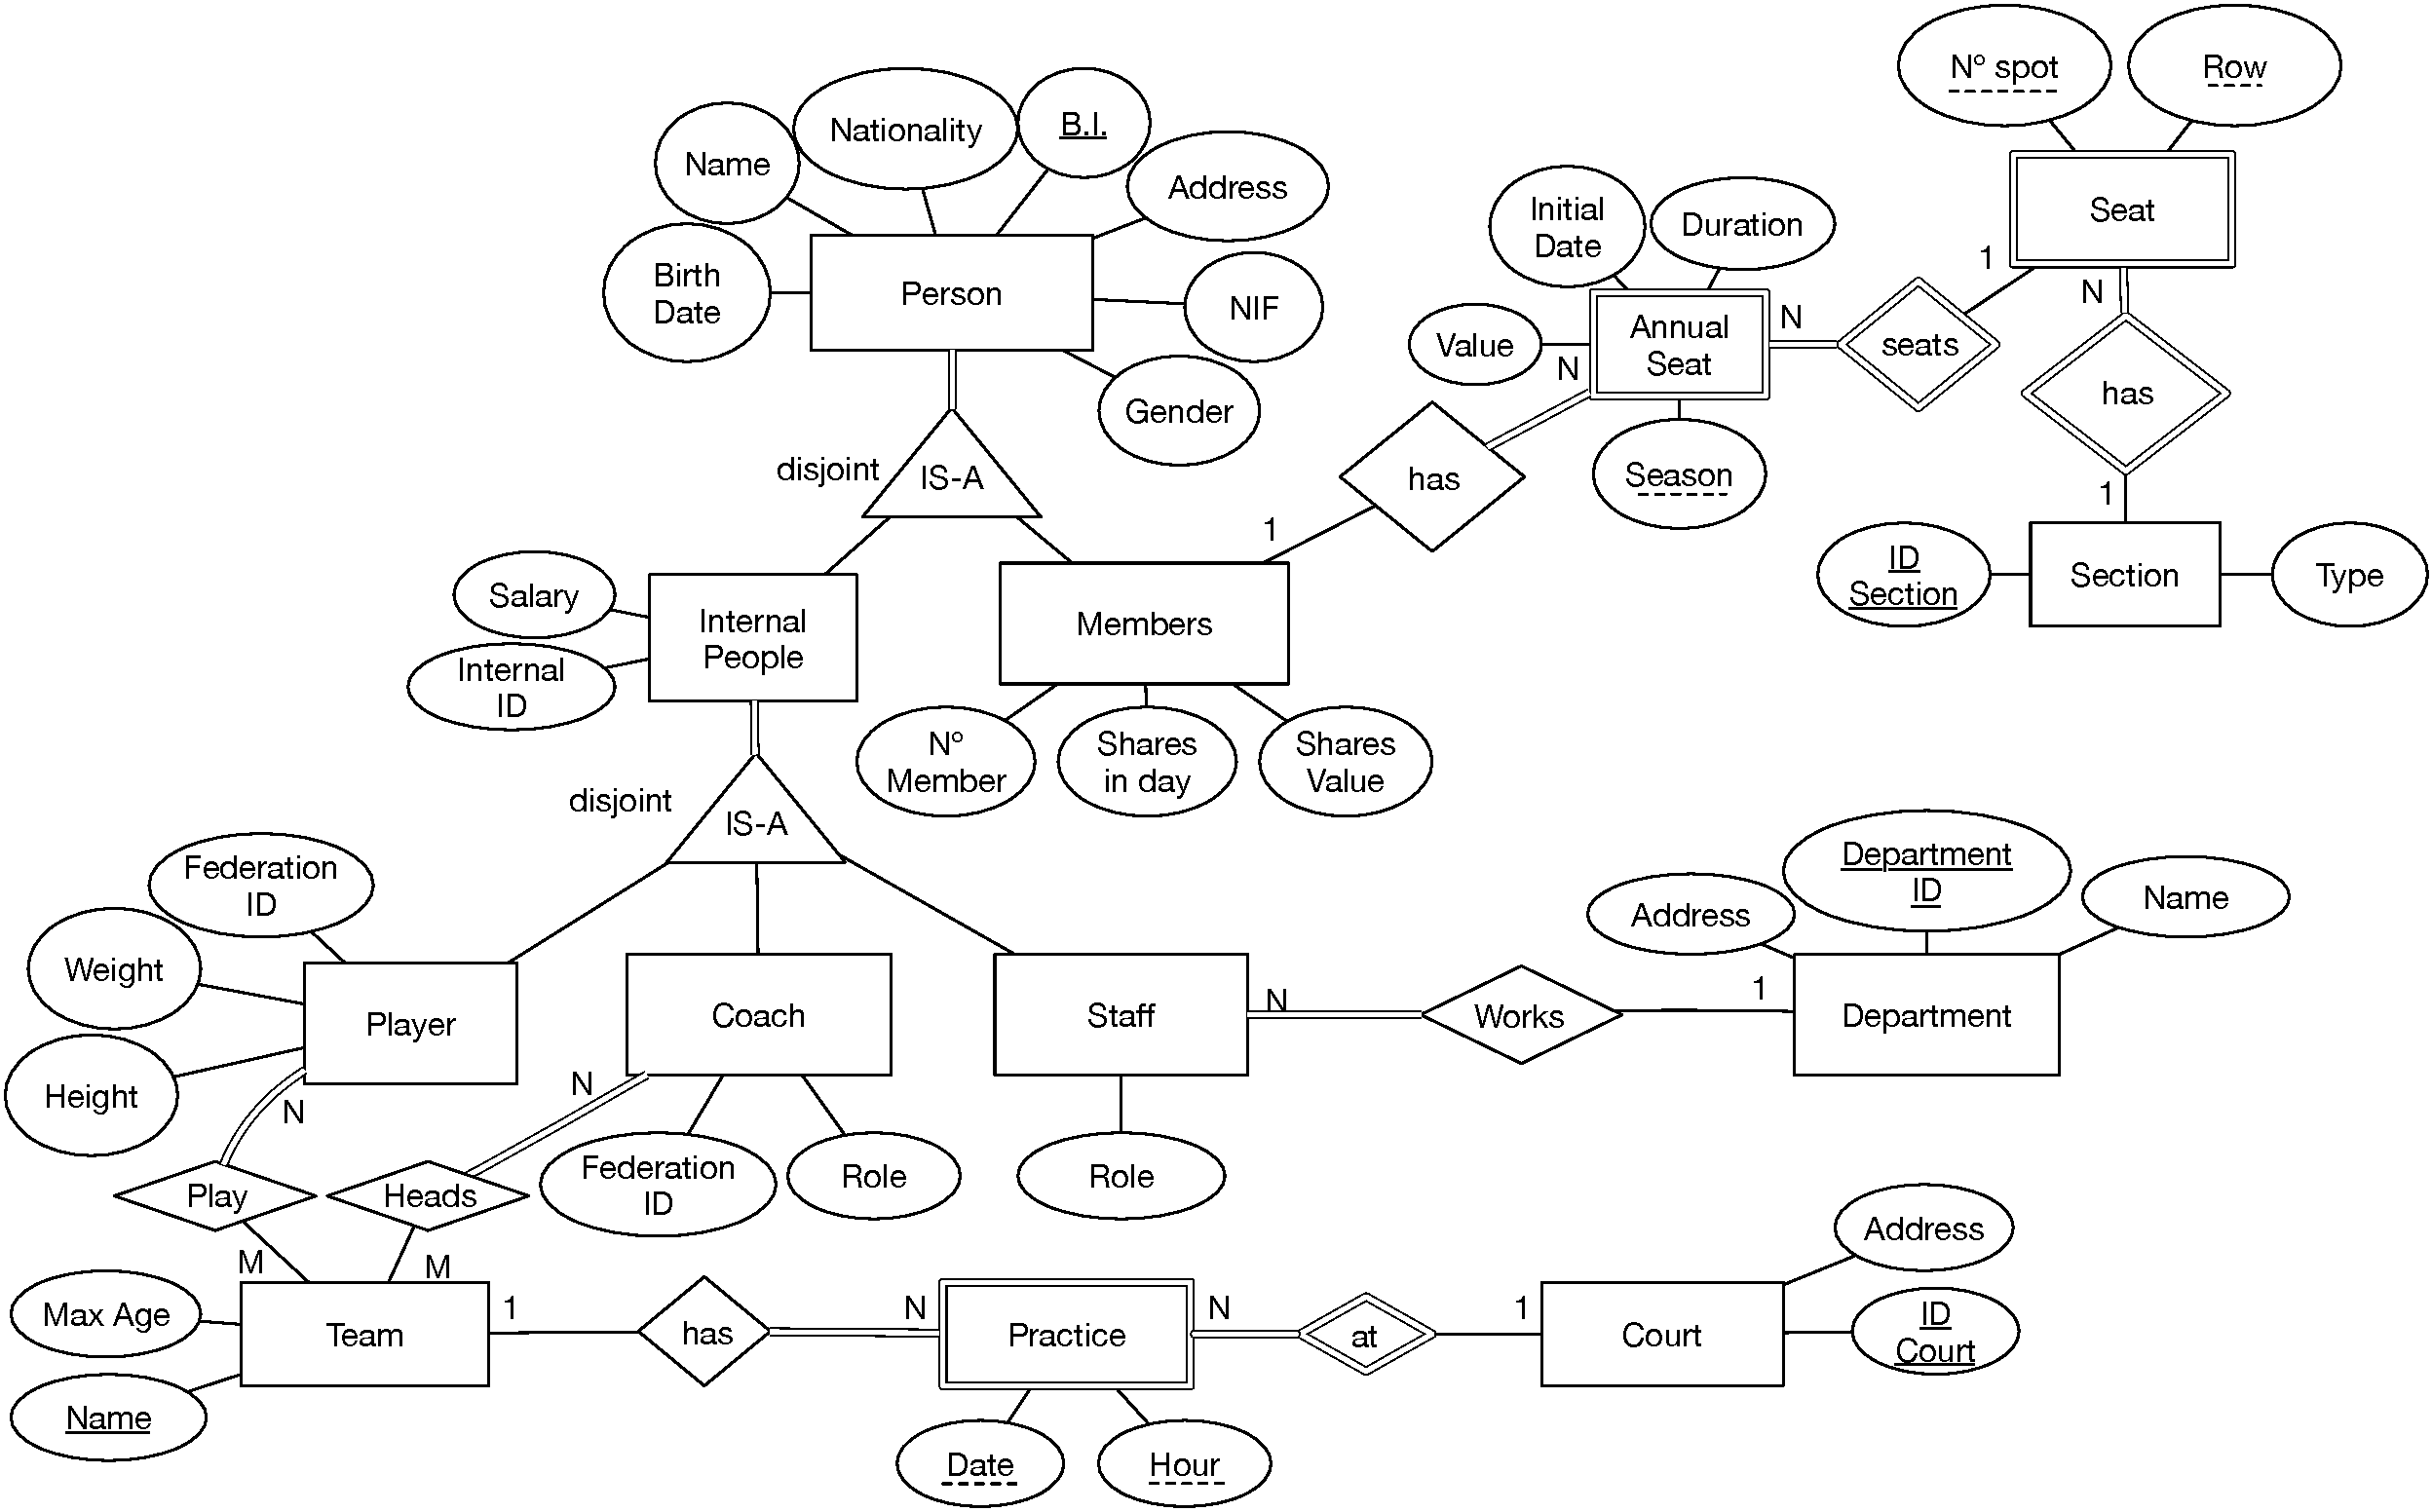
\includegraphics[width=135mm,scale=1]{EER.pdf}
 \caption{\\Diagrama entidade relação}\label{fig:eer}
\end{figure}

As entidades e os seus atributos correspondem à análise de requisitos realizada anteriormente. As relações são todas binárias.

\newpage
\section{Esquema Relacional da BD}
Após a construção do nosso desenho conceptual procedeu-se à elaboração do Modelo Relacional. Este modelo foi construído tendo por base o diagrama entidade relação e as regras para a realização desta tarefa. Cada entidade e cada relação irá gerar uma única tabela e após realizados os passos para conversão do desenho conceptual no modelo relacional 
foi criado o modelo relacional\ref{fig:mr}.

\begin{figure}[!htb]
 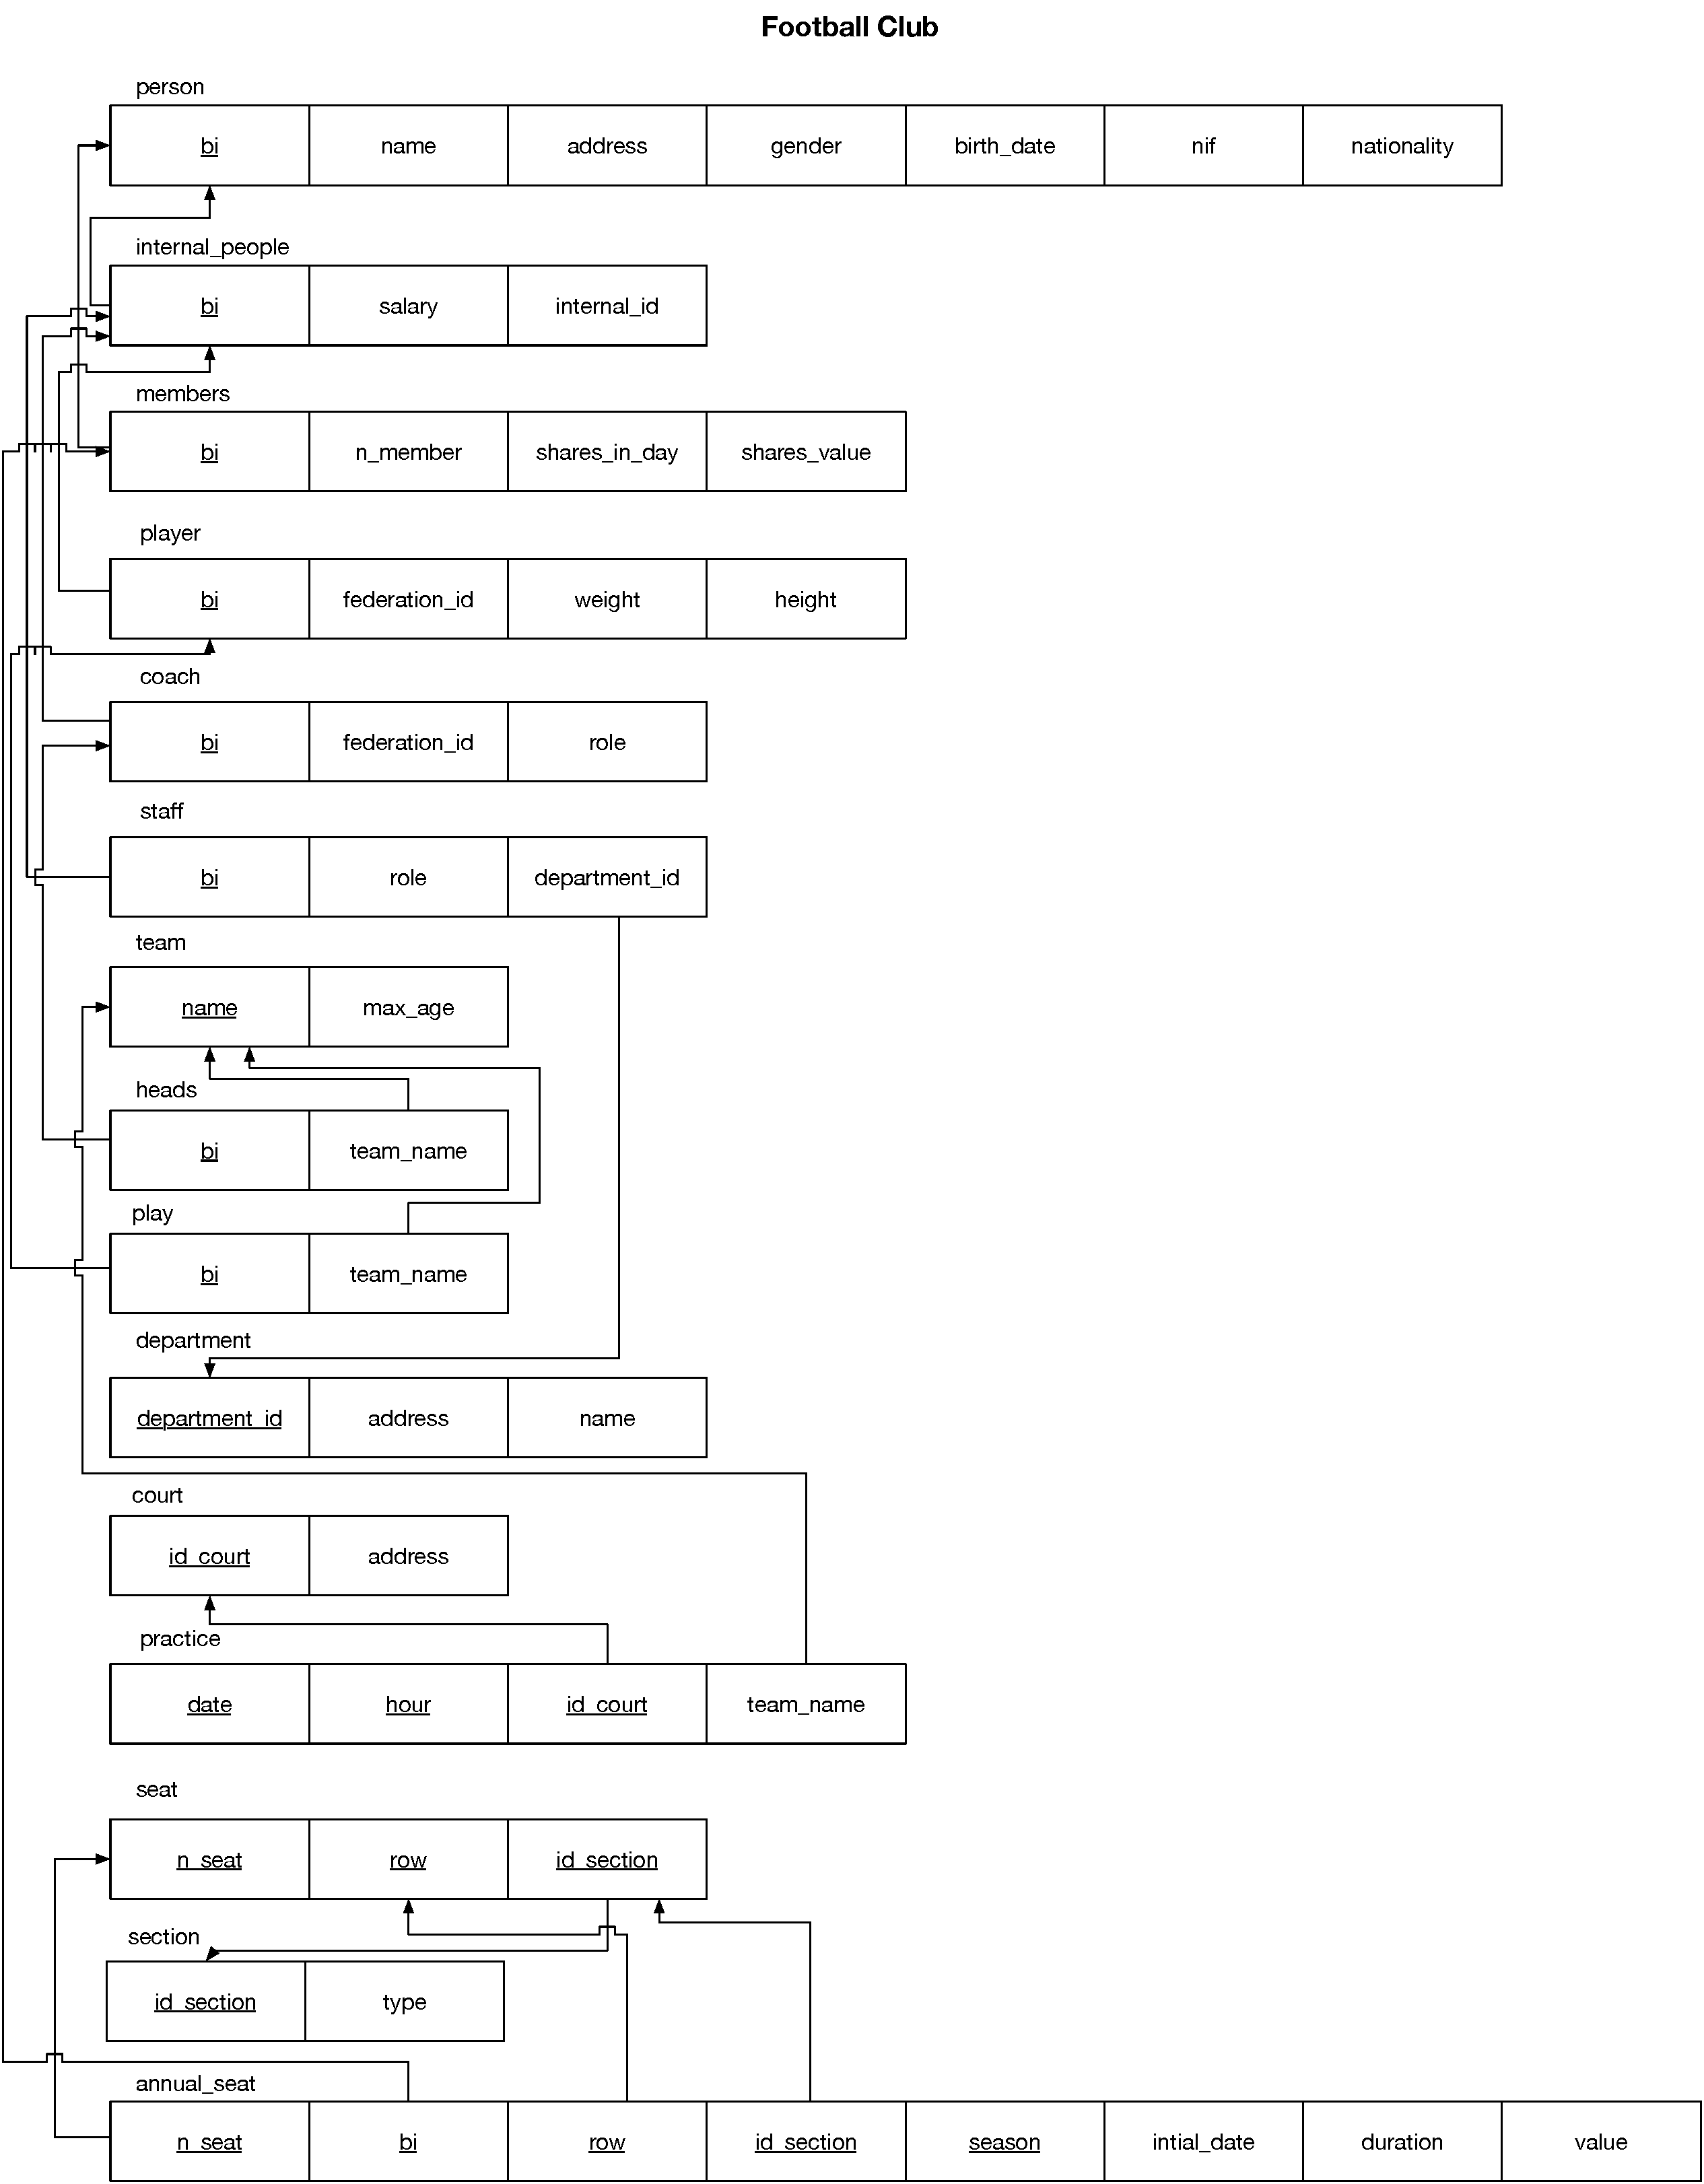
\includegraphics[width=115mm,scale=1]{modelo_relacional.pdf}
 \caption{\\Modelo relacional}\label{fig:mr}
\end{figure}

\newpage
\section{Normalização}
Para garantir a eficiência, a não existência de redundâncias e permitir a integridade referencial entre relações tive-se de usar normalizações.

Para realizar a normalização do nosso projeto teve-se em conta alguns conceitos. Inicialmente começa-se por garantir a 1FN, seguido da 2FN e usualmente terminando na 3FN. No entanto, em algumas situações a 3FN ainda apresenta algumas anomalias.
\\

Uma relação diz-se na 1FN quando:

- Os atributos são atómicos (simples e  indivisíveis), ou seja, não permite atributos composto ou multivalor.

- Não suporta relações dentro de relações, ou seja, não é possível utilizar uma relação como valor de um atributo de um tuplo.
\\

Uma relação diz-se na 2FN quando:

- Está na 1FN.

- Todos os atributos não pertencentes a qualquer chave candidata dependem totalmente da chave e não de parte dela.
\\

Uma relação diz-se na 3FN quando:

- Está na 2FN.

- Todos os atributos não chave não dependem funcionalmente uns dos outros, ou seja, são funcionalmente dependentes só e apenas da chave da relação.
\\

Uma relação diz-se na BCNF quando:

- Está na 3FN.

- Todos os atributos são funcionalmente dependentes da chave da relação, de toda a chave e de nada mais.
\\

Após a análise do nosso projecto pôde-se concluir que já se encontrava na 3FN pois não tem dependências transitivas e todos os atributos dependem da chave primária da sua relação.
\\

Como forma de demonstrar como foi realizada esta análise temos o seguinte exemplo:

\begin{figure}[!htb]
 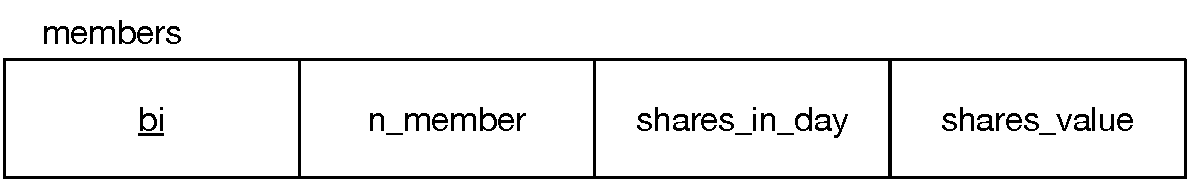
\includegraphics[width=40mm,scale=0.5]{exemplo_normalizacao.pdf}
\end{figure}

Neste exemplo temos a nossa relação Membro, que como pode-se verificar não existem atributos repetidos, multivalores ou compostos, estando assim na 1FN.

Esta relação também se encontra na 2FN, pois está na 1FN e todos os atributos dependem da chave primária da relação, ou seja, do BI.

Já está portanto na 3FN porque não tem dependências transitivas e todos os atributos dependem da chave primária.

\section{View's}
Foi decidido não usar views no desenvolvimento do nosso sistema. 

Em contra partida decidiu-se usar UDF's por estas serem mais seguras, serem compiladas e optimizadas, serem boas para ser utilizadas para incorporar lógica complexa dentro de uma consulta. 

As udf's também previnem a alteração ou remoção de objetos/tabelas utilizadas pela função.

Já as views não permitem esta camada de segurança, sendo assim, decidiu-se apenas usar UDF's para consulta de dados.

\newpage
\section{Índices}
Com o aumento do volume de dados, os pedidos de consulta começam a ter tempos de resposta maiores, pois os dados que existem nas tabelas encontram-se desorganizados. Para contrariar este aumento dos tempos de resposta devemos manter as tabelas organizadas de forma a que as consultas sejam efetuadas mais rapidamente. A utilização de índices nos campos que mais frequentemente serão utilizados é a maneira indicada, onde um ponteiro é criado para a posição real de cada registo.


Para tornar as nossas pesquisas mais eficientes introduzimos vários índices que achamos necessários (pesquisas feitas por dados não primários), do tipo NonClustered, pois os índices do tipo Clustered são automaticamente criados aquando da criação de uma tabela pois vai corresponder às chaves primárias.


Foram utilizados em todos os índices, um FILLFACTOR=75 com pad{\textunderscore}index, sendo que o primeiro determina a percentagem de espaço em cada página , quando um índice é criado, e o segundo, aplica às páginas de nível intermediário do índice a percentagem especificada pelo FILLFACTOR.
\\

Índice "indexactiveseat", exemplo:
\\

\begin{lstlisting}
go

CREATE NONCLUSTERED INDEX indexactiveseat ON football.seat(active)
WITH (FILLFACTOR=75,pad_index=ON);
\end{lstlisting}
 \vspace{0,5in}
Restantes índices estão disponíveis em anexo(ref):
\\


\newpage

\section{Stored Procedures}
Dicidiu-se usar stored procedures para criar uma camada de abstracção entre o modelo de dados, a sua manipulação e a camada aplicacional. A adopção desta abordagem permite-nos criar de forma segura, com boa performance e que garante a integridade dos dados, métodos para criar, modificar e apagar modelo de dados do nosso sistema de base de dados.

Outro dos motivos foi garantir um contrato de utilização entre o "developer" da aplicação e a utilização do nosso modelo de dados, permitindo assim especificar que parâmetros são necessários para realizar cada operação e garantindo também um bom controlo de erro avisando-o com T-SQL Raise Error quando este não estiver a cumprir o contrato.

As stored procedures ao contrário de um uso do nosso modelo de dados em DML permite que o conjunto de instruções compiladas na Stored Procedure  não tenham de ser recompiladas cada vez que o procedimento é invocado, sendo estas, apenas compiladas na primeira vez que são executadas e depois disso são guardadas em cache, sendo que isto permite maior rapidez no acesso ao modelo de dados.

Sendo assim, o principal foco em todas as stored procedures que se desenvolveu foi procurar garantir um bom controlo de erro para a camada aplicacional e que a criação, alteração ou remoção de dados do nosso modelo de dados fosse realizada de forma consistente.

De forma a garantir que as stored procedures responsáveis pela manipulação de dados em caso de erro na inserção de um grupo de instruções, os dados continuem consistentes  decidiu-se usar "Transactions".

\begin{lstlisting}
go 

CREATE PROCEDURE football.sp_createPlayer
  @bi				INT, 
  @name				VARCHAR(75),
  @address			VARCHAR(75), 
  @birth_date		DATE, 
  @nif				INT, 
  @gender			VARCHAR(1), 
  @nationality		VARCHAR(75),
  @salary			MONEY,
  @federation_id	INT,
  @weight			INT,
  @height			INT
WITH ENCRYPTION
AS 
	--Para garantir que todos os parametros enviados nao sao NULL decidiu-se garantir primeiro este contrato com um IF.
	 
	IF @bi is null OR @name is null OR @address is null OR @birth_date is null OR @nif is null OR 
		@gender is null OR @nationality is null OR @salary is null OR @federation_id is null OR
		@weight is null OR @height is null
	BEGIN
		-- Como este erro normalmente e causado pelo developer aplicacional optou-se por nao fazer um RAISE ERROR, contudo tambem poderia-se ter sido feito
		
		PRINT 'The bi, name, address, birth_date, nif, nationality, salary, federation_id, weight and height can not be null!'
		RETURN
	END
	
	DECLARE @count int

	-- Uma das restricoes no nosso modelo de dados e que nao podem existir pessoas com o mesmo BI, com este trexo de codigo garantimos isso e caso 
	-- check if the BI is already in use
	SELECT @count = count(bi) FROM football.person WHERE bi = @bi;

	IF @count != 0
	BEGIN
		RAISERROR ('The BI id is already in use!', 14, 1)
		RETURN
	END
		
	-- Nao faz sentido que um jogador e um treinador tenham o mesmo ID dentro da federacao, sendo assim tambem tem de ser comprido este contrato. Tambem se fez um Trigger para garantir este contrato num possivel manipulamento direto do modelo de dados
	
	-- check if the federation id is already in use
	SELECT @count = count(federation_id) FROM football.player WHERE federation_id = @federation_id;

	IF @count != 0
	BEGIN
		RAISERROR ('The federation id is already in use!', 14, 1)
		RETURN
	END
	
	-- check if the federation id is already in use
	SELECT @count = count(federation_id) FROM football.coach WHERE federation_id = @federation_id;

	IF @count != 0
	BEGIN
		RAISERROR ('The federation id is already in use by one coach!', 14, 1)
		RETURN
	END
	
	-- NIF e sempre unico
	
	-- check if the NIF is already in use
	SELECT @count = count(nif) FROM football.person WHERE nif = @nif;

	IF @count != 0
	BEGIN
		RAISERROR ('The NIF id is already in use!', 14, 1)
		RETURN
	END

	BEGIN TRANSACTION;
	
	--  Para garantir a integridade do nosso modelo de dados e necessario garantir que este conjunto de instrucoes sejam executadas e concluidas corretamente em conjunto e caso uma delas nao seja concluida com sucesso deve ser feito um RollBack garantindo assim que apenas serao inseridos dados de forma correta.
	
	BEGIN TRY
		INSERT INTO football.person 
					([bi], 
					 [name], 
					 [address], 
					 [birth_date], 
					 [nif], 
					 [gender],
					 [nationality]) 
		VALUES      ( @bi, 
					  @name, 
					  @address, 
					  @birth_date, 
					  @nif, 
					  @gender,
					  @nationality) 

		INSERT INTO football.internal_people 
					([bi], 
					 [salary]) 
		VALUES      ( @bi, 
					  @salary) 

		INSERT INTO football.player 
					([bi], 
					 [federation_id], 
					 [weight],
					 [height]) 
		VALUES      ( @bi, 
					  @federation_id, 
					  @weight,
					  @height)
		COMMIT TRANSACTION;
	END TRY
	BEGIN CATCH
		RAISERROR ('An error occurred when creating the player!', 14, 1)
		ROLLBACK TRANSACTION;
	END CATCH;

\end{lstlisting}
 \vspace{0,5in}

Restantes stored procedures estão disponíveis em anexo. (ref)

\newpage

\section{User-defined functions}
As UDF's no nosso modelo de dados desempenham o papel de vistas dado que não temos nenhuma "View". Uma user defined function representa várias vantagens em relação a uma view, podem ser usadas para incorporar lógica complexa numa pesquisa, podem aceitar parâmetros e usando schema binding previne a alteração ou remoção de objectos utilizados pela função.

Estas apresentam também a mesma característica do que os SPs por serem igualmente compilados e optimizados. Sendo assim o modelo de dados fica muito mais simples de ser usado e rápido.

Na maior parte das triggers optámos por uma lógica de quando os parâmetros de entrada fossem NULL a UDF retornaria todos os resultados da base de dados. Quando não fosse NULL ela retornaria resultados específicos.


\begin{lstlisting}
go

CREATE FUNCTION football.udf_players_data_grid(@team_name VARCHAR(50)=null)
RETURNS @table TABLE ("internal id" int, "bi" int, "name" varchar(75), "salary" money, "gender" varchar(1), "federation_id" int)
WITH SCHEMABINDING, ENCRYPTION
AS
BEGIN
	-- Quando @team_name e null mostra todos os jogadores de determinada equipa
	IF (@team_name is null)
		BEGIN
			INSERT @table SELECT	internal_people.internal_id AS 'internal id', person.bi, person.name, internal_people.salary, person.gender, player.federation_id AS 'federation id'
			FROM	(football.player JOIN (football.internal_people JOIN
football.person ON internal_people.bi = person.bi) ON player.bi = football.internal_people.bi);
		END;
		
	-- Quando @team_name nao e null entao mostra os detalhes de um jogador de determinada equipa
	ELSE
		BEGIN
			INSERT @table SELECT	internal_people.internal_id AS 'internal id', person.bi, person.name, internal_people.salary, person.gender, player.federation_id AS 'federation id'
			FROM	(football.play JOIN	(football.player JOIN (football.internal_people JOIN football.person ON internal_people.bi = person.bi) ON player.bi = football.internal_people.bi) ON play.bi = player.bi)
			WHERE team_name = @team_name;
		END;
	RETURN;
END;
\end{lstlisting}
 \vspace{0,5in}

Restantes user defined functions estão disponíveis em anexo. (ref)

\newpage
\section{Triggers}
De forma a garantir uma maior consistência e integridade da base de dados, foram utilizados alguns triggers. Estes são funções que são ativadas aquando de um insert, update ou delete numa determinada tabela de dados.

No nosso caso, foi criado, por exemplo, um  trigger que ocorre quando existe um pedido de delete na tabela "seat", este em vez de ser removido, altera o valor da variável "active" para 0 (INSTEAD OF).
O resto dos triggers utilizados resumem-se a verificações, no nosso caso, verificar se determinado "federation{\textunderscore}id" já existe aquando de um create ou de um update nas tabelas "coach" e "player".
Restantes triggers estão disponíveis em anexo(ref)
\\

\begin{lstlisting}
CREATE Trigger seatTrigger ON football.seat
INSTEAD OF DELETE
AS
	SET NOCOUNT ON;
	DECLARE @n_seat INT;
	DECLARE @row VARCHAR(1);
	DECLARE @id_Section INT;

	SELECT @n_seat = deleted.n_seat FROM deleted;
	SELECT @row = deleted.row FROM deleted;
	SELECT @id_section = deleted.id_section FROM deleted;
	
	-- Quando um pedido delete e executado na tabela football.seat, este trigger e ativado e em vez de apagar o "seat", altera a variavel "active" para o valor 0.
	
	BEGIN
		UPDATE football.seat SET
			   active = 0
			   WHERE seat.n_seat = @n_seat AND seat.row = @row AND seat.id_section = @id_section;
	END
\end{lstlisting}
 \vspace{0,5in}

\newpage
\section{Aplicação Utilizador}
A aplicação utilizador criada para este projecto, foi elaborada em conjunto com a disciplina de Interação Humano-Computador, em WPF/C\#.

Consiste num sistema de gestão de um clube de futebol, onde é possível efectuar as operações de inserção, alteração e remoção de entidades da Base de Dados, e ainda consultar estatísticas do clube.
\\

\begin{figure}[!htb]
 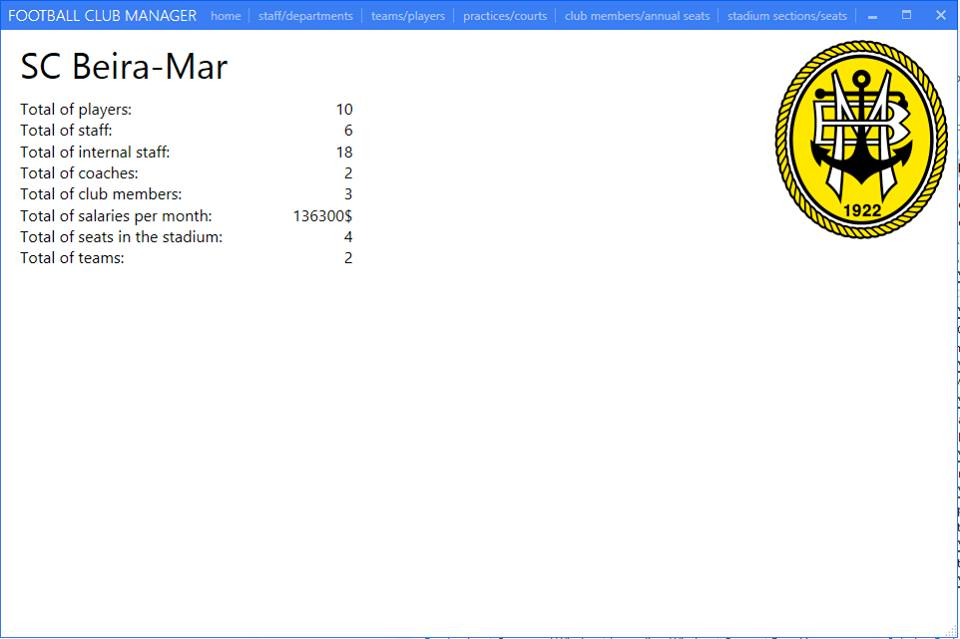
\includegraphics[width=135mm,scale=1]{app_home_page.jpg}
 \caption{\\Página Inicial}\label{fig:eer}
\end{figure}

\begin{figure}[!htb]
 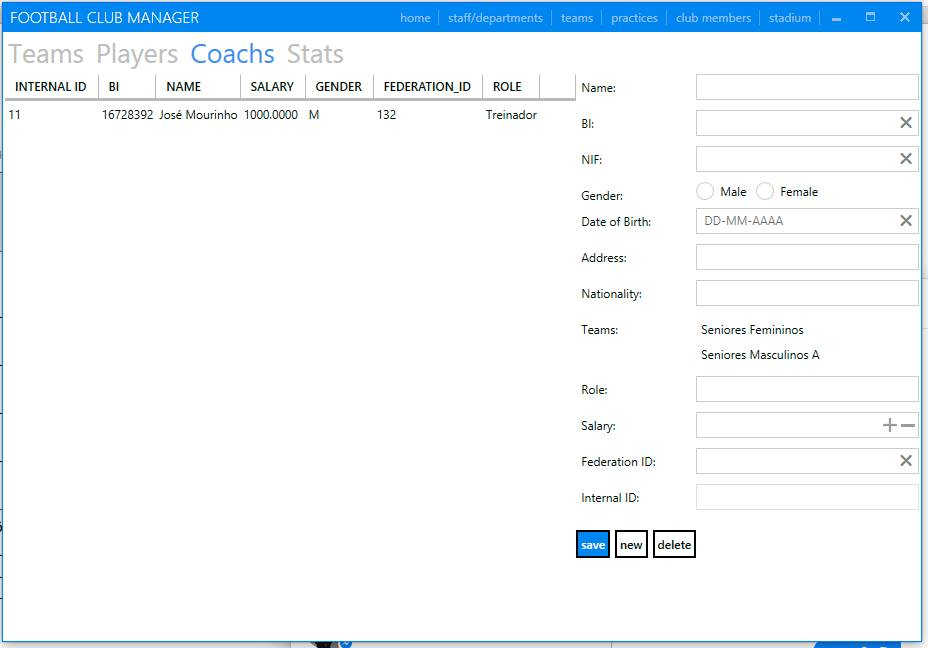
\includegraphics[width=135mm,scale=1]{app_add_coach.jpg}
 \caption{\\Página de listagem de Treinadores}\label{fig:eer}
\end{figure}


\clearpage
\section{Conclusão}
Os objectivos propostos foram alcançados, abordando grande parte dos conceitos leccionados na disciplina de Base de Dados, tanto na componente teórica como prática.
Foram efectuadas várias versões tanto do diagrama entidade-relação como do esquema relacional da Base de Dados, pois consoante se ia progredindo na elaboração do trabalho era necessário fazer alterações que se achassem necessárias.

Como foi referido neste relatório, a aplicação para o utilizador foi elaborada em conjunto com  a disciplina de Interação Humano-Computador, pelo que nos permitiu utilizar os conhecimentos adquiridos nesta mesma disciplina em WPF/C\#.

Concluindo, foi um trabalho bastante útil para o nosso desenvolvimento enquanto estudantes da área de Engenharia de Computadores e Telemática, pois permitiu a prática dos conceitos adquiridos na disciplina de Base de Dados.

\newpage
\section{Referências}

\begin{itemize}
	\item Mahapps - http://mahapps.com/ 
	\item Protection from SQL Injection http://programming-review.com/stop-mysql-injection/ 
	\item Data Grid selected http://blog.scottlogic.com/2008/12/02/wpf-datagrid-detecting-clicked-cell-and-row.html 
	\item Data Grid http://www.codeproject.com/Articles/30905/WPF-DataGrid-Practical-Examples\#displaying 
	\item Slides das aulas teóricas
\end{itemize}


\newpage
\section{Anexos}
Em anexo a este relatório anexou-se uma pasta com todos os SQL usados para este sistema.

\end{document}